\subsection{Pengujian Pengiriman Citra}
\label{subsec:imagetransfertesting}

\begin{figure} [ht]
  \centering
  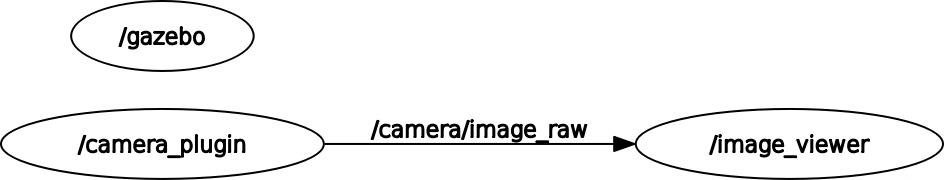
\includegraphics[width=0.45\textwidth]{figures/rosgraph/image-transfer-sim.png}
  \IfLanguageName{english}{
    \caption{Node scheme of the image transfer testing in the simulation.}
  }{
    \caption{Skema \emph{node} dari pengujian pengiriman citra di simulasi.}
  }
  \label{fig:rosgraphimagetransfersim}
\end{figure}

\begin{figure} [ht]
  \centering
  
\includegraphics[width=0.45\textwidth]{figures/rosgraph/image-transfer-real.png}
  \IfLanguageName{english}{
    \caption{Node scheme of the image transfer testing in the real robot.}
  }{
    \caption{Skema \emph{node} pengujian pengiriman citra pada \emph{real robot}.}
  }
  \label{fig:rosgraphimagetransferreal}
\end{figure}


Pengujian pengiriman citra dilakukan dengan menjalankan \emph{node} \lstinline{image_viewer} yang akan menampilkan citra yang diterima dalam bentuk GUI.
Seperti yang terlihat pada gambar \ref{fig:rosgraphimagetransfersim},
  di simulasi,
  \emph{node} \lstinline{image_viewer} akan terhubung dengan \emph{node} \lstinline{camera_plugin} yang akan mengirimkan data citra melalui \emph{topic} \lstinline{/camera/image_raw}.
Sedangkan untuk pengujian di dunia nyata,
  seperti yang terlihat pada gambar \ref{fig:rosgraphimagetransferreal},
  peran dari \emph{node} \lstinline{camera_plugin} akan digantikan oleh \emph{node} \lstinline{v4l2_camera} yang akan mengirimkan data citra yang berasal dari device camera yang ada pada robot fisik.


\begin{figure}[ht]
  \centering
  \begin{tikzpicture}
    \begin{axis}[
        height=0.2\textwidth,
        width=0.45\textwidth,
        xlabel=\IfLanguageName{english}{Data Size}{Ukuran Data} (KB),
        ylabel=\IfLanguageName{english}{Delay}{\emph{Delay}} (ms),
        legend style={
          at={(0.5,1.5)},
          anchor=north,
          legend columns=-1,
        },
        ymajorgrids,
        ymin=0,
        ymax=125,
      ]
      \addplot table[x=size,y=delay,col sep=comma]{data/image-transfer-sim.csv};
      \addplot table[x=size,y=delay,col sep=comma]{data/image-transfer-bd-sim.csv};
      \IfLanguageName{english}{
        \legend{Same Device, Between Device}
      }{
        \legend{Sesama Perangkat, Antar Perangkat}
      }
    \end{axis}
  \end{tikzpicture}
  \IfLanguageName{english}{
    \caption{Delay results of image transfer in the simulation.}
  }{
    \caption{Hasil \emph{delay} dari pengiriman citra di simulasi.}
  }
  \label{fig:imagetransferdelaysim}
\end{figure}


\begin{figure}[ht]
  \centering
  \begin{tikzpicture}
    \begin{axis}[
        height=0.2\textwidth,
        width=0.45\textwidth,
        xlabel=\IfLanguageName{english}{Data Size}{Ukuran Data} (KB),
        ylabel=\IfLanguageName{english}{Rate}{Frekuensi} (hz),
        legend style={
          at={(0.5,1.5)},
          anchor=north,
          legend columns=-1,
        },
        ymajorgrids,
        ymin=0,
        ymax=40,
      ]
      \addplot table[x=size,y=rate,col sep=comma]{data/image-transfer-sim.csv};
      \addplot table[x=size,y=rate,col sep=comma]{data/image-transfer-bd-sim.csv};
      \IfLanguageName{english}{
        \legend{Same Device, Between Device}
      }{
        \legend{Sesama Perangkat, Antar Perangkat}
      }
    \end{axis}
  \end{tikzpicture}
  \IfLanguageName{english}{
    \caption{Rate results compared to the data size of image transfer in the simulation.}
  }{
    \caption{Hasil frekuensi dibandingkan ukuran data dari pengiriman citra di simulasi.}
  }
  \label{fig:imagetransferratesim}
\end{figure}


Pengujian pengiriman citra dilakukan pada kondisi pengiriman pada perangkat yang sama dan pada pengiriman antara dua perangkat yang berbeda.
Pengujian tersebut masing-masing dilakukan dengan berbagai macam kombinasi nilai resolusi dari 160x120 hingga 1920x1080 pada robot virtual di lingkungan simulasi maupun pada robot fisik di dunia nyata.
Seperti yang terlihat pada gambar \ref{fig:imagetransferdelaysim} dan gambar \ref{fig:imagetransferratesim},
  di simulasi,
  nilai \emph{delay} yang dihasilkan cenderung naik sedangkan nilai frekuensi yang dihasilkan cenderung turun seiring dengan besarnya data yang dikirimkan.
Dari hasil tersebut,
  hingga resolusi 800x600 ($\pm2500$ KB),
  pengiriman citra di simulasi mampu menghasilkan \emph{delay} rendah di bawah 50 ms dan frekuensi stabil di atas 90\% dari nilai normalnya.


\begin{figure}[ht]
  \centering
  \begin{tikzpicture}
    \begin{axis}[
        height=0.2\textwidth,
        width=0.45\textwidth,
        xlabel=\IfLanguageName{english}{Data Size}{Ukuran Data} (KB),
        xlabel=\IfLanguageName{english}{$K^{th}$ Attempt}{Percobaan Ke-$K$},
        legend style={
          at={(0.5,1.5)},
          anchor=north,
          legend columns=-1,
        },
        ymajorgrids,
        ymin=0,
        ymax=125,
      ]
      \addplot table[x=size,y=delay,col sep=comma]{data/image-transfer-real.csv};
      \addplot table[x=size,y=delay,col sep=comma]{data/image-transfer-bd-real.csv};
      \IfLanguageName{english}{
        \legend{Same Device, Between Device}
      }{
        \legend{Sesama Perangkat, Antar Perangkat}
      }
    \end{axis}
  \end{tikzpicture}
  \IfLanguageName{english}{
    \caption{Delay results of image transfer on the real robot.}
  }{
    \caption{Hasil \emph{delay} dari pengiriman citra pada robot fisik.}
  }
  \label{fig:imagetransferdelayreal}
\end{figure}


\begin{figure}[ht]
  \centering
  \begin{tikzpicture}
    \begin{axis}[
        height=0.2\textwidth,
        width=0.45\textwidth,
        xlabel=\IfLanguageName{english}{Data Size}{Ukuran Data} (KB),
        ylabel=\IfLanguageName{english}{Rate}{Frekuensi} (hz),
        legend style={
          at={(0.5,1.5)},
          anchor=north,
          legend columns=-1,
        },
        ymajorgrids,
        ymin=0,
        ymax=40,
      ]
      \addplot table[x=size,y=rate,col sep=comma]{data/image-transfer-real.csv};
      \addplot table[x=size,y=rate,col sep=comma]{data/image-transfer-bd-real.csv};
      \IfLanguageName{english}{
        \legend{Same Device, Between Device}
      }{
        \legend{Sesama Perangkat, Antar Perangkat}
      }
    \end{axis}
  \end{tikzpicture}
  \IfLanguageName{english}{
    \caption{Rate results compared to the data size of image transfer on the real robot.}
  }{
    \caption{Hasil frekuensi dibandingkan ukuran data dari pengiriman citra pada robot fisik.}
  }
  \label{fig:imagetransferratereal}
\end{figure}


Sedangkan,
  pada robot fisik,
  seperti yang terlihat pada gambar \ref{fig:imagetransferdelayreal} dan gambar \ref{fig:imagetransferratereal},
  hasil yang didapatkan juga relatif sama dimana nilai \emph{delay} cenderung naik sedangkan nilai frekuensi cenderung turun.
Namun,
  berbeda dengan hasil pengujian di lingkungan simulasi,
  dari hasil pada robot fisik tersebut,
  didapatkan bahwa hingga resolusi 640x480 ($\pm1500$ KB),
  pengiriman citra pada robot real mampu menghasilkan \emph{delay} rendah di bawah 50 ms dan frekuensi stabil di atas 90\% dari nilai normalnya.
